\documentclass[11pt, oneside]{article}   	% use "amsart" instead of "article" for AMSLaTeX format
\usepackage{geometry}                		% See geometry.pdf to learn the layout options. There are lots.
\geometry{letterpaper}                   		% ... or a4paper or a5paper or ... 
%\geometry{landscape}                		% Activate for rotated page geometry
\usepackage[parfill]{parskip}    		% Activate to begin paragraphs with an empty line rather than an indent
\usepackage{graphicx}				% Use pdf, png, jpg, or eps§ with pdflatex; use eps in DVI mode
								% TeX will automatically convert eps --> pdf in pdflatex		
\usepackage{amssymb}
\usepackage{booktabs}
\usepackage[procnames]{listings}
\usepackage{color}
\title{Practical 3:\\
 Predicting Music Tastes}
\author{Samuel Daulton, Taylor Killian, and Andrew Petschek (ML Marauders)}
%\date{}							% Activate to display a given date or no date

\begin{document}
\maketitle
\section{Technical Approach}

In this practical we were provided data that contained the profile information of about 233,000 users of a music streaming service along with a collection of the number of times that each user listened to the songs of 2,000 different artists. We were provided the objective of learning the relationship between users to the degree to enable the prediction of any given user's listening habits. That is, if supplied with a user/artist pair, report an estimate of how many times that user would listen to that artist. 

In this section we outline the methods by which we familiarized ourselves with the data. We highlight some key insights gained through data exploration, discuss how we addressed these issues and how they informed our initial modeling attempts. 

\subsection{Data Exploration}

The primary purpose of our initial data exploration was to understand how the user profiles varied, the key characteristics of these users as well as how their total plays were distributed. We believed that by gaining greater insight into the data, we would develop intuition of how to achieve the objective of predicting the number of user plays. There were two primary hurdles in parsing the data toward meeting our objective. Both of these initial challenges derive from instances of the provided data being incomplete or broadly distributed. User profile information (unique ID, gender, age and country) was self-reported and as a result some of the fields were missing for some users. The other source of missing data was that none of the users listened to every artist. On average a user listened to approximately 18 artists out of the set of 2,000 provided to us, with the most number of artists listened to being 47 (see Fig.~\ref{fig:hist_artists_listenedto}). Further analysis of the missing information in the user profile data is completed in Sec.~\ref{sec:filling_data}.

\begin{figure}[ht!]
\centering
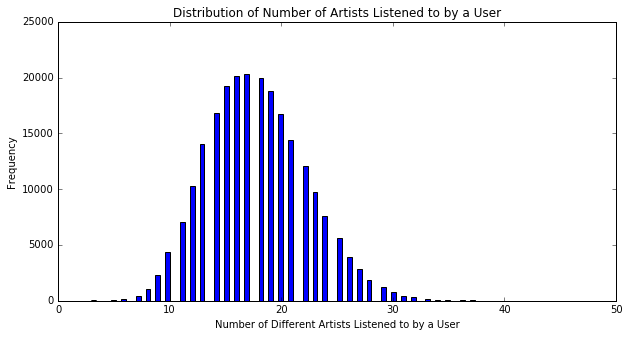
\includegraphics[width=0.95\textwidth]{images/artists_listenedto.png}
\caption{Histogram representing number of artists each user listened to in the provided data.}
\label{fig:hist_artists_listenedto}
\end{figure} 

When investigating the total number of plays each user accrued (Fig.~\ref{fig:num_plays_per_user}) we noticed that the distribution is heavily skewed to the left in a Poisson-like manner with an drawn out tail. What this represents is that it is increasingly unlikely that any user in the provided data set would listen to an artist more than 500 times. The variance of total plays across these users is so large that there is no discernible mass in the distribution of the play totals. This presented a significant issue for us when we tried to cluster the data according to kNN and k-means algorithms, which will be detailed in Sec.~\ref{sec:modeling}.

\begin{figure}[ht!]
\centering
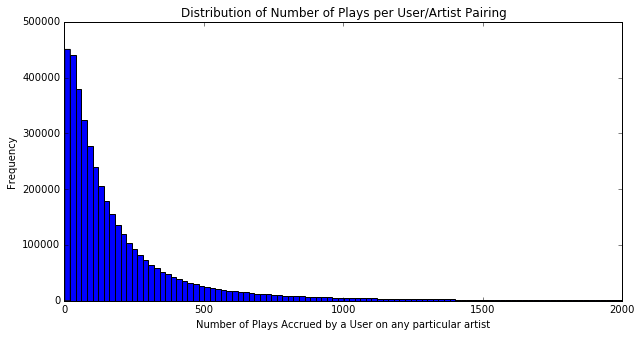
\includegraphics[width=0.95\textwidth]{images/plays_per_user.png}
\caption{Histogram representing number of plays each user accrued in the provided data. For visualization purposes, we have excluded any values higher than 2000.}
\label{fig:num_plays_per_user}
\end{figure} 



\subsection{Filling in Missing Values}
\label{sec:filling_data}

At first, we approached this practical in terms of a collaborative filtering problem, taking the Netflix challenge as our motivation. In order to begin that process, we needed to complete the user profile data so that we could adequately cluster similar users, using profile information, under the assumption that individuals of similar gender, age and country would potentially share music preferences. We felt that, of these three features, age would be the greatest discriminator and so we set out to fill in the ages of all users. When exploring the different ages supplied by the users we found that close to 45,000 users didn't supply an age when creating an account. We also found that there were 625 registered users with ages greater than 100 and a further 650 users with age less than 8 (including a grouping of users with age = -1337). We removed all of these seemingly spoofed ages and set out to treat these users as though they didn't supply an age.

In order to fill in the age of each user, we set out to use as much information as we had available for each user. We clustered those users from the same country of the same gender as each user that was missing an age, as that information was available. In the event that a user didn't provide country or gender information, we supplied them with the median age of the user database.  

\begin{figure}[ht!]
\centering
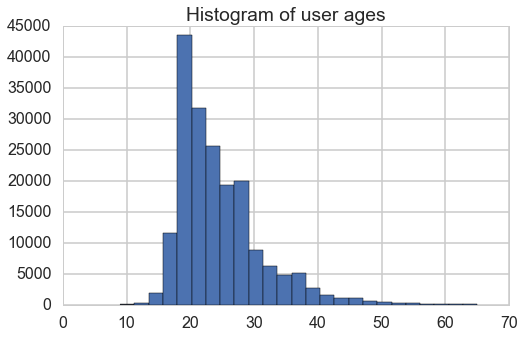
\includegraphics[width=0.45\textwidth]{images/ages.png} \quad 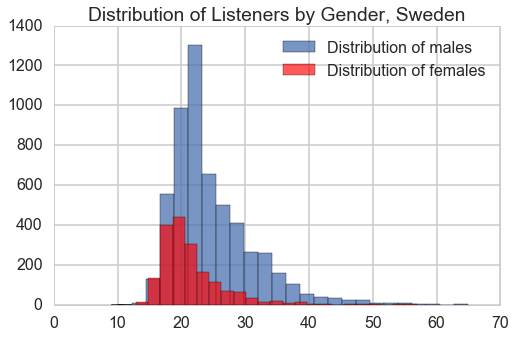
\includegraphics[width=0.45\textwidth]{images/ages_sweden.png}
\caption{Representative histograms of ages of general user database (l) and ages, filtered by country and gender (r), the medians from which were used to fill in a user's age.}
\label{fig:age_histograms}
\end{figure} 

\subsection{Feature Engineering} 

To fill out the feature vector of each user we collected mean and median measurements of each users plays per artist and per genre. We acquired the genres of the artists in our database by scraping the information from the MusicBrainz database. Along with these means and medians we recorded the number of unique artists a user listened to. We also created indicator variables for each country, gender and whether or not there was missing information in a users profile. The hope was that these indicators would serve to segment the data and enable easier clustering when applying k-means or kNN.

\subsection{Initial Attempts}\label{sec:initial_attempts}

We wanted to construct a baseline for predicting how many times a user $u$ would listen to an artist $a$ that outlined $u$'s tendency to listen to music more or less than the general population (user median plays per artist, $\bar{Y}_u$ vs. the global median $\bar{Y}$). We also wanted to account for the median plays of similar users (conditioned on them having listened to $a$) compared to the global median based on users in the same age range ($\bar{Y}_{age|a}$), who were of the same gender ($\bar{Y}_{g|a}$) and/or who were from the same country ($\bar{Y}_{c|a}$) as $u$.

This baseline prediction for user $u$, given artist $a$ was modeled as:

$$Plays_{u|a} = \bar{Y} + (\bar{Y}-\bar{Y}_u) + (\bar{Y}-\bar{Y}_{age|a}) + (\bar{Y}-\bar{Y}_{s|a})+ (\bar{Y}-\bar{Y}_{c|a})  $$

The aim of what we called Bias Summation was to adjust the naive predictions based on only global and user median play counts by accounting for users of similar demographic profile to user $u$ and how they chose to listen to artist $a$. We later wanted to extend this method and augment the above sum by comparing how the median number of plays from user $u$ compared to users of similar demographics, not conditioned on any artist, but ran out of time.

Another initial attempt we made was to use the two baselines and compute a weighted average between them. This weight was computed based on the number of unique artists each user listened to. Our reasoning was that if a user hadn't listened to many artists, there wouldn't be much information to form a prediction and the median value for number of plays wouldn't be as informative. In contrast, if a user had listened to many artists, we would feel more confident in using their median values of plays for a prediction. Thus, we computed the following predictions for each user without regard to artist: $$Plays_{u} = \left(\frac{1}{n}\right)\bar{Y} + \left(1 - \frac{1}{n}\right)\bar{Y}_u$$ where n is the number of artists, user $u$ listened to.

\section{Results}

As summarized in Sec.~\ref{sec:initial_attempts} and Sec.~\ref{sec:modeling}, we tried a variety of methods and heuristics to predict a user's number of plays for a particular artist after aggregating user data according to demographic information. These approaches were oftentimes computationally prohibitive within the time frame of the practical, according to our implementation. The results of these various methods and approaches are summarized in Table 1.


\begin{table}[]
\centering
\label{table:results}
\begin{tabular}{@{}ll@{}}
\toprule
\textbf{Model} & \textbf{MAE (Public Score)} \\ \midrule
Weighted Average between Global and User Medians & 137.77885\\
\\
{\bf Per-user Median} & 137.79146\\
\\
SGD Regression using Huber Loss & 144.60821 \\
Linear Regression on Means/Medians using L-2 Loss &  160.23209 \\
%Unbiased Estimators & 168.03096\\
Ensemble Regression of k-means with Means/Medians  &  181.02842\\
Bias Summation & 189.57480\\
\\
{\bf Global Median} & 201.78204\\
\\
kNN on Genres & N/A\\
kNN on Profile Data & N/A\\
NMF & N/A\\

\bottomrule
\end{tabular}
\caption{Model Results}
\end{table}

\section{Modeling Techniques with Discussion}\label{sec:modeling}

Our general techniques proceeded with the following structure:
\begin{itemize}
\item Aggregate similar users via heuristic or clustering method
\item Compare general measurements like means/medians and other quantitative features
\item Regress against these features to formulate a prediction based on similar user data
\end{itemize}

The methods that we used and were familiar with to aggregate data was in Pandas and Spark. We created large dataframes of the training data. With these large data structures, we had a difficult time successfully implementing any methods of sklearn confidently. We tested several clustering techniques on small subsets of the data to gauge how long they would take to run (with our implementation) on the test set. We quickly found that the computation time needed to completely predict on the test set was prohibitive (kNN methods as well as naive Matrix Factorization). We also encountered times where our results against a validation subset, set aside from our training data, of our data were so poor that they didn't warrant use in predicting against the test set.

\subsection{Bias Summation}

Outlined above in Sec.~\ref{sec:initial_attempts}. This method provided a MAE of 189.57480 which served to improve our predictions above the baseline for the global median but was disappointingly far from the user median baseline. 

\subsection{Weighted Average Between Global and User Medians}

Also outlined in Sec.~\ref{sec:initial_attempts}. This method provided our best MAE score, 137.77885, which was above the Per-User Median baseline. We were happy to see that our weighting approach based on the number of artists a user listened to was valid in that it adjusted our predictions to be slightly more accurate than the baseline, showing that in some cases, the Global median was a better predictor.

\subsection{k Nearest Neighbors}

We tried two separate approaches when trying to evaluate the k nearest neighbors of any particular user. The first based on demographic information and generic features such as number of artists listened to as well as the user's median plays. The other approach with kNN was to find similar users based on the specific artists listened to by each user, including genre. When implementing these methods on our training set, we realized that they took too long to run. Performing them on the test set would have been according to our implementation.

\subsection{k-Means Clustering}

In order to perform k-Means clustering we standardized the data in our training set, both indicator variables and the number of plays of each artist by subtracting the mean and dividing by the standard deviation. The concept that we followed was that as a user was assigned to any particular cluster, the artist for whom we are predicting plays would take on the median value of the cluster mean for that artist. Due to sparsity, this resulted into biasing our data against the highest value for plays in the data set which was often significantly greater than the median number of plays per artist. The result of this standardization, and by finding 25 clusters, was that the predicted number of plays for most user, artist pairing was set to zero even after rescaling the prediction by adding in the mean and multiplying by the standard deviation. This wasn't a very effective implementation and as such we received a MAE score of 181.02842. We felt that if we had more clusters we would be able to closer approximate a users number of listens as we would have a tighter fit of similar users in each cluster. We started a run, looking for 1000 clusters but early diagnostics showed that we would have needed 200 hours for the clustering to be completed on the training data. Time we didn't have.
	
\subsection{Regression against means and medians}

We wanted to investigate the relationship between the means and medians of different quantitative measure of each user's music preferences, those of the user database as a whole as well as other users listening activity for the artist that we're trying to predict for the particular user. We performed two different kinds of regressions based on the loss function we hoped to optimize. The first regression was generic Linear Regression with L-2 loss. This performed worse than we expected (160.23209 MAE) on the test set which led us to investigate other loss functions. We determined that minimizing the sum of squared errors wasn't the best method as the evaluative metric used in the kaggle competition was that of absolute error.

We settled on running Stochastic Gradient Descent using Huber loss. We decided on Huber loss because it was designed to be a piecewise approximation between squared loss and absolute loss, which is a closer representation of the kaggle evaluation metric. We figured that by attempting to minimize this loss while applying regression techniques would better approximate the data we were given and how our methods were evaluated. This piecewise definition of the loss function is also more robust against outliers and otherwise non-smooth/discrete data. Our performance improved over regression using L-2 loss, achieving a decrease of close to 16 points (144.60821 MAE).

\subsection{Matrix Factorization}

We tried to apply sklearn's built in Matrix Factorization code to fill in the missing values of the training data from which we could pull off the test predictions. This idea was derived from trying to follow the development of a collaborative filtering approach. Our implementation was computationally prohibitive however, only processing a small proportion of our test data in several hours. We abandoned this approach soon after realizing the strain it would put on our ability to accomplish anything else for this practical.

\section{Summary}

NEED TO FILL THIS IN!!!!

\newpage
\section{Code}

\definecolor{keywords}{RGB}{255,0,90}
\definecolor{comments}{RGB}{0,0,113}
\definecolor{red}{RGB}{160,0,0}
\definecolor{green}{RGB}{0,150,0}
 
\lstset{language=Python, 
        basicstyle=\ttfamily\small, 
        keywordstyle=\color{keywords},
        commentstyle=\color{comments},
        stringstyle=\color{red},
        showstringspaces=false,
        identifierstyle=\color{green},
        procnamekeys={def,class}}
 
\begin{lstlisting}

# Load libraries
import numpy as np
import matplotlib.pyplot as plt
import pandas as pd
import pickle
from time import time
from sklearn import linear_model
from sklearn.cross_validation import train_test_split
from sklearn.neighbors import KNeighborsRegressor
from sklearn.preprocessing import StandardScaler
import warnings
import math
from sklearn.cluster import KMeans
from sklearn.decomposition import NMF
import pickle
from sklearn.externals import joblib
warnings.filterwarnings('ignore')
%matplotlib inline

# load default data frames
train_df = pd.read_csv("train.csv")
test_df = pd.read_csv("test.csv")
artists_df = pd.read_csv("artists.csv")
global_median_df = pd.read_csv("global_median.csv")
profiles = pd.read_csv("profiles_AJP.csv")

# CREATES PROFILES DF

# # condition = (profiles_df['age'].isnull()) | (profiles_df['age'] < 95) | (profiles_df['age'] > 0)
# # profiles_df[condition] = np.nan
# profiles_df.loc[profiles_df["age"] < 5 ,'age'] = None
# profiles_df.loc[profiles_df["age"] > 85 ,'age'] = None
# profiles_df.loc[profiles_df["age"].isnull(),'age'] = None

# # calculate mean age per user
# mean_age = profiles_df[~profiles_df['age'].isnull()]["age"].mean()

# ###################################################################### 

# # calculate mean age per men
# males_only_df = profiles_df[profiles_df["sex"]=='m']
# mean_male_age = males_only_df[~males_only_df['sex'].isnull()]["age"].mean()

# ###################################################################### 

# # calculate mean age per women
# females_only_df = profiles_df[profiles_df["sex"]=='f']
# mean_female_age = females_only_df[~females_only_df['sex'].isnull()]["age"].mean()

# ###################################################################### 

# # get list of unique countries
# countries = profiles_df["country"].unique()

# # calculate mean age per country
# mean_country_age = {}
# for country in countries:
#     tmp_df = profiles_df[profiles_df["country"]==str(country)].copy()
#     mean_country_age[str(country)] = tmp_df["age"].mean()

# ###################################################################### 
    
# # calculate mean age per male per country
# mean_country_male_age = {}
# for country in countries:
#     tmp_df0 = profiles_df[profiles_df["sex"]=='m'].copy()
#     tmp_df1 = tmp_df0[profiles_df["country"]==str(country)].copy()
#     mean_country_male_age[str(country)] = tmp_df1["age"].mean()

# ###################################################################### 

# # calculate mean age per female per country
# mean_country_female_age = {}
# for country in countries:
#     tmp_df0 = profiles_df[profiles_df["sex"]=='f'].copy()
#     tmp_df1 = tmp_df0[profiles_df["country"]==str(country)].copy()
#     mean_country_female_age[str(country)] = tmp_df1["age"].mean()

# ###################################################################### 

# # initialize training df
# profiles = profiles_df

# ###################################################################### 

# # create sex indicators
# profiles["male"] = 0
# profiles["female"] = 0
# profiles["sex_missing"] = 0
# profiles.loc[profiles["sex"] =='m', "male"] = 1
# profiles.loc[profiles["sex"] =='f', "female"] = 1
# profiles.loc[profiles["sex"].isnull(), "sex_missing"] = 1

# ######################################################################  

# # create age indicators
# profiles["age_missing"] = 0
# profiles.loc[profiles["age"].isnull(),"age_missing"] = 1

# # fill in mean age: has no gender or country
# profiles.loc[profiles["age_missing"] == 1, "age"] = mean_age

# # fill in mean age: has gender, no country
# #males
# condition = (profiles["sex"] =='m') & (profiles["country"].isnull()) & (profiles["age_missing"] == 1)
# profiles.loc[condition, "age"] = mean_male_age
# # females
# condition = (profiles["sex"] =='f') & (profiles["country"].isnull()) & (profiles["age_missing"] == 1)
# profiles.loc[condition, "age"] = mean_female_age

# # fill in mean age: has country, no gender
# #loop over countries
# for country in countries:
#     condition = (profiles["country"] == country) & (profiles["age_missing"] == 1) & (profiles["sex_missing"] == 1)
#     profiles.loc[condition, "age"] = mean_country_age[country]

# # fill in mean age: has gender and country
# # loop over countries
# for country in countries:
#     # males
#     condition = (profiles["country"] == country) & (profiles["sex"] == 'm') & (profiles["age_missing"] == 1)
#     profiles.loc[condition, "age"] = mean_country_male_age[country]
#     # females
#     condition = (profiles["country"] == country) & (profiles["sex"] == 'f') & (profiles["age_missing"] == 1)
#     profiles.loc[condition, "age"] = mean_country_female_age[country]

# ###################################################################### 
    
# # create country indicators
# profiles["country_missing"] = 0
# profiles.loc[profiles["country"].isnull(), "country_missing"] = 1
# # loop over countries
# for country in countries:
#     # assign 1 if in that country
#     profiles.loc[profiles["country"] == country, country] = 1
#     # assign 0 otherwise
#     profiles.loc[profiles["country"] != country, country] = 0

# ###################################################################### 

# profiles.to_csv("profiles.csv")

# ###################################################################### 

# clean profiles df
profiles.drop("sex",inplace=True,axis=1)
profiles.drop("country",inplace=True,axis=1)
profiles.drop("Unnamed: 0",axis=1,inplace=True)
profiles.set_index("user",inplace=True)
profiles.drop("sex_missing",inplace=True,axis=1)
#profiles.head(1)

profiles.reset_index(inplace=True)

# # if SMALL DF
# profile_features = ["age","male","female","age_missing","United States","Germany","United Kingdom","France","Poland","Brazil","Spain","Italy"]
# num_profile_features = len(profile_features)
# sm_profiles = profiles.loc[:,profile_features]
# sm_profiles.reset_index(inplace=True)
# #sm_profiles.head(1)

# load genre data frames and do some cleaning
artists_with_1genre_df = pd.read_csv("artists_with_genres.csv")
artists_with_5genres_df = pd.read_csv("artists_with_top_5_genres.csv")
artists_with_5genres_df.rename(columns = {"num_votes5":"extra"}, inplace = True)
artists_with_5genres_df.rename(columns = {"genre5":"num_votes5"}, inplace = True)
artists_with_5genres_df.rename(columns = {"num_votes4":"genre5"}, inplace = True)
artists_with_5genres_df.rename(columns = {"genre4":"num_votes4"}, inplace = True)
artists_with_5genres_df.rename(columns = {"num_votes3":"genre4"}, inplace = True)
artists_with_5genres_df.rename(columns = {"genre3":"num_votes3"}, inplace = True)
artists_with_5genres_df.rename(columns = {"num_votes2":"genre3"}, inplace = True)
artists_with_5genres_df.rename(columns = {"genre2":"num_votes2"}, inplace = True)
artists_with_5genres_df.rename(columns = {"num_votes1":"genre2"}, inplace = True)
artists_with_5genres_df.rename(columns = {"genre1":"num_votes1"}, inplace = True)
artists_with_5genres_df.rename(columns = {"name":"genre1"}, inplace = True)
artists_with_5genres_df.rename(columns = {"artist":"name"}, inplace = True)

# Calculate percent of votes
agn = artists_with_5genres_df[["num_votes1","num_votes2","num_votes3"]]
agn.rename(columns = {"num_votes1":"per_votes1"}, inplace = True)
agn.rename(columns = {"num_votes2":"per_votes2"}, inplace = True)
agn.rename(columns = {"num_votes3":"per_votes3"}, inplace = True)
agn = agn.apply(lambda c: c / c.sum() * 100, axis=1)

del artists_df

# combine dfs together
artists_with_5genres_df = pd.concat([artists_with_5genres_df, agn], axis=1)
#artists_with_5genres_df.head(1)

# Train - Test Split on profiles to ensure users are in one group or another
train, valid = train_test_split(train_df, test_size = .001)
#train, valid = train_test_split(train0, test_size = .1)
#train = train_df.copy()

#add primary genre to train
train["genre1"] = np.nan
train.set_index("artist", inplace=True)
train.update(artists_with_5genres_df)
train.reset_index(inplace=True)

# test["genre1"] = np.nan
# test.set_index("artist", inplace=True)
# test.update(artists_with_5genres_df)
# test.reset_index(inplace=True)

valid["genre1"] = np.nan
valid.set_index("artist", inplace=True)
valid.update(artists_with_5genres_df)
valid.reset_index(inplace=True)

# train0["genre1"] = np.nan
# train0.set_index("artist", inplace=True)
# train0.update(artists_with_5genres_df)
# train0.reset_index(inplace=True)

#add primary genre to train
train["genre1"] = np.nan
train.set_index("artist", inplace=True)
train.update(artists_with_5genres_df)
train.reset_index(inplace=True)

# test["genre1"] = np.nan
# test.set_index("artist", inplace=True)
# test.update(artists_with_5genres_df)
# test.reset_index(inplace=True)

valid["genre1"] = np.nan
valid.set_index("artist", inplace=True)
valid.update(artists_with_5genres_df)
valid.reset_index(inplace=True)

# train0["genre1"] = np.nan
# train0.set_index("artist", inplace=True)
# train0.update(artists_with_5genres_df)
# train0.reset_index(inplace=True)

# calculate user medians
user_medians = train.pivot(index='user',columns='artist',values='plays').reset_index().set_index('user').median(axis=1)
user_medians = pd.DataFrame(user_medians)
user_medians.rename(columns={0:"user median"},inplace=True)
#user_medians.head(1)

# calculate user means
user_means = train.pivot(index='user',columns='artist',values='plays').reset_index().set_index('user').mean(axis=1)
user_means = pd.DataFrame(user_means)
user_means.rename(columns={0:"user mean"},inplace=True)
#user_means.head(1)

# calculate artist medians
artist_medians = train.pivot(index='user',columns='artist',values='plays').reset_index().set_index('user').median(axis=0)
artist_medians = pd.DataFrame(artist_medians)
artist_medians.rename(columns={0:"artist median"},inplace=True)
#artist_medians.head(1)

# calculate artist medians
artist_means = train.pivot(index='user',columns='artist',values='plays').reset_index().set_index('user').mean(axis=0)
artist_means = pd.DataFrame(artist_means)
artist_means.rename(columns={0:"artist mean"},inplace=True)
#artist_means.head(1)

# calculate genre medians
genre_medians = train.groupby("genre1").plays.median()
genre_medians = pd.DataFrame(genre_medians)
genre_medians.rename(columns={'plays':"genre median"},inplace=True)
#genre_medians.head(1)

# calculate genre mean
genre_means = train.groupby("genre1").plays.mean()
genre_means = pd.DataFrame(genre_means)
genre_means.rename(columns={'plays':"genre mean"},inplace=True)
#genre_means.head(1)

# calculate genre_user medians
user_genre_medians = train.groupby(["user","genre1"]).median().reset_index()
user_genre_medians.rename(columns={"plays": "user genre median"},inplace=True)
#user_genre_medians.head(1)

# calculate genre_user means
user_genre_means = train.groupby(["user","genre1"]).mean().reset_index()
user_genre_means.rename(columns={"plays": "user genre mean"},inplace=True)
#user_genre_means.head(1)

#pivot training data to have one row per user
train = train.pivot(index='user',columns='artist',values='plays').reset_index()
train = train.fillna(0)

# BIG PROFILE
#get index for later
users = profiles.user
profiles.set_index('user', inplace=True)
# fill in any missing values just in case
profiles[profiles.age.isnull()]=profiles.age.mean()

# standardize profile data
# scaler = StandardScaler()
# profiles_scaled = pd.DataFrame(scaler.fit_transform(profiles))
# cols = profiles.columns
# profiles_scaled.columns = cols
# profiles_scaled.index = users

# combine profile and training data
bigdf = pd.concat([profiles,train],axis=1,join_axes=[profiles.index])
#bigdf.head(1)

num_profile_features = len(profiles.columns)

# # SMALL PROFILE IF KNN
# #join profiles and train together
# train.set_index('user',inplace = True)
# #train.head(1)

# # get index for later
# users = sm_profiles.user
# sm_profiles.set_index('user', inplace=True)
# # fill in any missing values just in case
# sm_profiles[sm_profiles.age.isnull()]=sm_profiles.age.mean()

# # standardize profile data
# scaler = StandardScaler()
# sm_profiles_scaled = pd.DataFrame(scaler.fit_transform(sm_profiles))
# cols = sm_profiles.columns
# sm_profiles_scaled.columns = cols
# sm_profiles_scaled.index = users

# # combine profile and training data
# bigdf = pd.concat([sm_profiles_scaled,train],axis=1,join_axes=[sm_profiles_scaled.index])
# #bigdf.head(1)

bigdf.fillna(0,inplace=True)
neigh = KNeighborsRegressor(n_neighbors=1000, weights="uniform")
%time neigh.fit(bigdf.iloc[:,:num_profile_features],bigdf.iloc[:,num_profile_features:])

# use this function in APPLY for a df
def knn_median_predict(test_row,avg):

    # get artist and user info
    artist = test_row[0]
    user = test_row[1]  

    # grab row from bigdf to test
    to_test = bigdf.iloc[bigdf.index == user,:num_profile_features]

    # grab indices of neighbors in bigdf
    idx = neigh.kneighbors(to_test)[1][0]
    predictions = np.array([bigdf.ix[iix,artist] for iix in idx])
    
    # get median from the k=1,3,5 nearest (non-zero) neighbors
    if avg == "median":
        return np.median(predictions[np.nonzero(predictions)][:1]),np.median(predictions[np.nonzero(predictions)][:3]),np.median(predictions[np.nonzero(predictions)][:5])
    else:
         return np.mean(predictions[np.nonzero(predictions)][:1]),np.mean(predictions[np.nonzero(predictions)][:3]),np.mean(predictions[np.nonzero(predictions)][:5])
        

valid["knn median"] = None
%time valid["knn median"] = valid.iloc[:,:].apply(lambda x: knn_median_predict(x,"median"),axis=1)

%time valid[['knn1 median', 'knn3 median', 'knn5 median']] = valid['knn median'].apply(pd.Series)

user_medians.values.reshape([user_medians.shape[0],1]).shape

user_medians_r = user_medians.values.reshape([user_medians.shape[0],1])
for i in range(num_profile_features,2245):
    mask = bigdf.iloc[:,i].values == 1102.5
    bigdf.iloc[:,i][mask] = user_medians_r[mask]
    print "\r" + str(i),

scaler = StandardScaler()
bigdf_sc = pd.DataFrame(scaler.fit_transform(bigdf))

# carry out kmeans
kmeans = KMeans(init = 'k-means++', n_clusters=1000, n_jobs = -1, n_init = 6)
%time kmeans.fit(bigdf_sc)

joblib.dump(kmeans, 'kmeans50.pkl') 

cols = bigdf.columns
centers = pd.DataFrame(scaler.inverse_transform(kmeans.cluster_centers_))
centers.columns = cols
centers.head()

closest_centers = kmeans.predict(bigdf_sc)
valid['closest center'] = closest_centers.tolist()
valid['closest center'] = None
valid.set_index("user",inplace=True)
valid.update(train)
valid.reset_index(inplace=True)

def get_prediction(x):
    artist = x[1]
    return centers.ix[x[5],artist]

valid["kmeans pred"] = 0
valid["kmeans pred"] = valid.apply(lambda x: get_prediction(x),axis=1)
valid.head()

# initialize columns
valid['user genre median'] = np.nan
valid['user median'] = np.nan
valid['artist median'] = np.nan
valid['genre median'] = np.nan
valid['global median'] = np.nan
valid['user mean'] = np.nan
valid['genre mean'] = np.nan
valid['artist mean'] = np.nan
valid['user genre mean'] = np.nan

# add global median
valid['global median'] = global_median

# add user median
valid.set_index('user',inplace=True)
valid.update(user_medians)
valid.reset_index(inplace=True)

# add artist median
valid.set_index('artist',inplace=True)
valid.update(artist_medians)
valid.reset_index(inplace=True)
valid["genre median"].fillna(valid["user median"],inplace=True)

# add genre median
valid.set_index('genre1',inplace=True)
valid.update(genre_medians)
valid.reset_index(inplace=True)
valid["genre median"].fillna(valid["user median"],inplace=True)

# add user genre median
valid.set_index(['user','genre1'],inplace=True)
valid.update(user_genre_medians.set_index(["user","genre1"]))
valid.reset_index(inplace=True)
valid["user genre median"].fillna(valid["user median"],inplace=True)

# add user mean
valid.set_index('user',inplace=True)
valid.update(user_means)
valid.reset_index(inplace=True)

# add artist mean
valid.set_index('artist',inplace=True)
valid.update(artist_means)
valid.reset_index(inplace=True)
valid["genre mean"].fillna(valid["user mean"],inplace=True)

# add genre mean
valid.set_index('genre1',inplace=True)
valid.update(genre_means)
valid.reset_index(inplace=True)
valid["genre mean"].fillna(valid["user mean"],inplace=True)

# add user genre mean
valid.set_index(['user','genre1'],inplace=True)
valid.update(user_genre_means.set_index(["user","genre1"]))
valid.reset_index(inplace=True)
valid["user genre mean"].fillna(valid["user mean"],inplace=True)
valid.head(1)

print valid.isnull().sum()

valid.loc[valid['knn1 median'].isnull(),'knn1 median'] = valid.loc[valid['knn1 median'].isnull(),"user median"]
valid.loc[valid['knn3 median'].isnull(),'knn3 median'] = valid.loc[valid['knn3 median'].isnull(),"user median"]
valid.loc[valid['knn5 median'].isnull(),'knn5 median'] = valid.loc[valid['knn5 median'].isnull(),"user median"]

# weighted ensemble
stacking= linear_model.LinearRegression()

X = np.vstack([valid['knn1 median'].values,valid['knn3 median'].values])
X = np.vstack([X,valid['knn5 median'].values])
X = np.vstack([X,valid['user median'].values])
X = np.vstack([X,valid['user genre median'].values])
X = np.vstack([X,valid['genre median'].values])
X = np.vstack([X,valid['artist median'].values])
X = np.vstack([X,valid['user mean'].values])
X = np.vstack([X,valid['user genre mean'].values])
X = np.vstack([X,valid['artist mean'].values])
X = np.vstack([X,valid['genre mean'].values])


X = X.T

y = valid['plays'].values

stacking.fit(X,y)
stacking.coef_

valid['ensemble'] =                            \
stacking.coef_[0]*valid['knn1 median']           \
+ stacking.coef_[1]*valid['knn3 median']         \
+ stacking.coef_[2]*valid['knn5 median']         \
+ stacking.coef_[3]*valid['user median']       \
+ stacking.coef_[3]*valid['user genre median'] \
+ stacking.coef_[4]*valid['genre median']      \
+ stacking.coef_[5]*valid['artist median']     \
+ stacking.coef_[6]*valid['user mean']     \
+ stacking.coef_[7]*valid['user genre mean']     \
+ stacking.coef_[8]*valid['artist mean']     \
+ stacking.coef_[9]*valid['genre mean']     \

valid['AE'] = np.abs(valid['plays']-valid['ensemble']) 
print "MAE is:", valid.AE.mean()

test = test_df.copy()

test["genre1"] = np.nan
test.set_index("artist", inplace=True)
test.update(artists_with_5genres_df)
test.reset_index(inplace=True)

# initialize columns
test['user genre median'] = np.nan
test['user median'] = np.nan
test['artist median'] = np.nan
test['genre median'] = np.nan
test['global median'] = np.nan
test['user mean'] = np.nan
test['genre mean'] = np.nan
test['artist mean'] = np.nan
test['user genre mean'] = np.nan

# add global median
test['global median'] = global_median

# add user median
test.set_index('user',inplace=True)
test.update(user_medians)
test.reset_index(inplace=True)

# add artist median
test.set_index('artist',inplace=True)
test.update(artist_medians)
test.reset_index(inplace=True)
test["genre median"].fillna(test["user median"],inplace=True)

# add genre median
test.set_index('genre1',inplace=True)
test.update(genre_medians)
test.reset_index(inplace=True)
test["genre median"].fillna(test["user median"],inplace=True)

# add user genre median
test.set_index(['user','genre1'],inplace=True)
test.update(user_genre_medians.set_index(["user","genre1"]))
test.reset_index(inplace=True)
test["user genre median"].fillna(test["user median"],inplace=True)

test["knn1 pred"] = None
%time test["knn1 pred"] = test.apply(lambda x: knn_profile_predict(x,1),axis=1)
test["knn3 pred"] = None
%time test["knn3 pred"] = test.apply(lambda x: knn_profile_predict(x,3),axis=1)
test["knn5 pred"] = None
%time test["knn5 pred"] = test.apply(lambda x: knn_profile_predict(x,5),axis=1)

test['ensemble'] =                            \
stacking.coef_[0]*test['knn1 pred']         \
+ stacking.coef_[1]*test['knn3 pred']         \
+ stacking.coef_[2]*test['knn5 pred']         \
+ stacking.coef_[3]*test['user median']       \
+ stacking.coef_[4]*test['user genre median'] \
+ stacking.coef_[5]*test['genre median']      \
+ stacking.coef_[6]*test['artist median']     \
# + stacking.coef_[7]*vvalid['global median']     \
# + stacking.coef_[8]*vvalid['user mean']
# + stacking.coef_[9]*vvalid['user genre mean']   \
# + stacking.coef_[10]*vvalid['genre mean']        \
# + stacking.coef_[11]*vvalid['artist mean']      

output_for_kaggle = test
output_for_kaggle.drop(["plays","closest center", "AE", "genre1","user","artist","knn pred","knn1 pred","knn3 pred","knn5 pred","user genre median","user median", "genre median", "global median","artist median","artist mean","user mean", "genre mean", "user genre mean"],axis=1,inplace=True)
output_for_kaggle.rename(columns={"ensemble":"plays"},inplace = True)
output_for_kaggle.head()

import numpy as np
import csv
import pandas as pd

# Create helper function to fill in missing ages based on country and gender (if available)
def fill_ages(indf):
    '''This helper function takes in a cleaned dataframe (with columns: user, age, sex and country)
    where invalid ages have been replaced with null values. This function infers a user's age based
    on their country and gender. If one or both of those is missing, the inference is performed on 
    the most informative subset of the data we have (at worst this is the entire dataset).'''
    # First copy dataframe for safety's sake
    outdf = indf.copy()
    
    # Loop through the entries in the data frame that have null valued age
    for index, (user_id,gender,age,country) in indf[indf.age.isnull()].iterrows():
        
        # Build up conditions over which we're calculating distribution of ages for this particular user
        #nans won't equal themselves
        if gender != gender:       # gender is not present
            if country != country: # country isn't present either
                
                condition = (~indf.age.isnull())
            else:
                
                condition = (~indf.age.isnull()) & (~indf.sex.isnull()) & (indf.country == country)
        elif country != country:   # country isn't present
            
            condition = (~indf.age.isnull()) & (indf.sex == gender)
        else:                      # both are present
            
            condition = (~indf.age.isnull()) & (indf.sex == gender) & (indf.country == country)
        
        # Extract array of ages relevant to the current user, based on country and gender (if available)
        relevant_ages = np.array(indf.age[condition]).astype('int64')
        relevant_ages_aggregated = np.bincount(relevant_ages)
        # Normalize to create a distribution (assuming that it's continuous between low and high (no need for pseudocounts))
        normed_ages = relevant_ages_aggregated/float(np.sum(relevant_ages_aggregated))
        
        # Found that there are some edge cases where there are few users from nation x that all have no age... 
        # Recalculate distribution
        if len(normed_ages) == 0: 
            if gender != gender:
                condition = (~indf.age.isnull()) & (~indf.sex.isnull())
            else:
                condition = (~indf.age.isnull()) & (indf.sex == gender)
            relevant_ages = np.array(indf.age[condition]).astype('int64')
            relevant_ages_aggregated = np.bincount(relevant_ages)
            normed_ages = relevant_ages_aggregated/float(np.sum(relevant_ages_aggregated))
            
        # Randomly assign user age based on distribution
        new_age = np.random.choice(range(len(normed_ages)),size=1,replace=True,p=normed_ages)[0]
        outdf.loc[index,'age'] = new_age
    
    # Return filled dataframe
    return outdf


if __name__ == '__main__':
	# Load user profiles
	user_databasedf = pd.read_csv("profiles.csv")

	# Create copy to remove spurrious ages (anything less than 10 and above 65)
	fixed_age_databasedf = user_databasedf.copy()
	fixed_age_databasedf.loc[(user_databasedf.age <= 8) | (user_databasedf.age > 65),'age'] = None

	# Fill values of missing age
	completed_age_databasedf = fill_ages(fixed_age_databasedf)
	completed_age_databasedf.to_csv("complete_age_profiles.csv")

import numpy as np
import csv
import matplotlib.pyplot as plt
# Predict via the user-specific median.
# If the user has no data, use the global median.

train_file = 'train.csv'
test_file  = 'test.csv'
soln_file  = 'user_median.csv'

# Load the training data.
train_data = {}
# key = user, value = number of artists that the user listened to
num_diff_artists = {}
with open(train_file, 'r') as train_fh:
    train_csv = csv.reader(train_fh, delimiter=',', quotechar='"')
    next(train_csv, None)
    for row in train_csv:
        user   = row[0]
        artist = row[1]
        plays  = row[2]
    
        if not user in train_data:
            train_data[user] = {}
            num_diff_artists[user] = 0.0
        
        train_data[user][artist] = int(plays)
        num_diff_artists[user] += 1

# Plot histogram of number of artists that a user listened to
plt.hist(num_diff_artists.values,bins=100)
plt.show()

# Compute the global median and per-user median.
plays_array  = []
user_medians = {}
for user, user_data in train_data.iteritems():
    user_plays = []
    for artist, plays in user_data.iteritems():
        plays_array.append(plays)
        user_plays.append(plays)

    user_medians[user] = np.median(np.array(user_plays))
global_median = np.median(np.array(plays_array))

# Write out test solutions.
with open(test_file, 'r') as test_fh:
    test_csv = csv.reader(test_fh, delimiter=',', quotechar='"')
    next(test_csv, None)

    with open(soln_file, 'w') as soln_fh:
        soln_csv = csv.writer(soln_fh,
                              delimiter=',',
                              quotechar='"',
                              quoting=csv.QUOTE_MINIMAL)
        soln_csv.writerow(['Id', 'plays'])

        for row in test_csv:
            id     = row[0]
            user   = row[1]
            artist = row[2]


            if user in user_medians:
                n = num_diff_artists[user]
                prediction  = 1.0/n * global_median + (1-1.0/n) * user_medians[user]
                soln_csv.writerow([id, prediction])
            else:
                print "User", id, "not in training data."
                soln_csv.writerow([id, global_median])

import numpy as np
import csv
import matplotlib.pyplot as plt
# Predict via the user-specific median.
# If the user has no data, use the global median.

train_file = 'train.csv'
test_file  = 'test.csv'
soln_file  = 'user_median.csv'

# Load the training data.
train_data = {}
train_plays = []
# key = user, value = number of artists that the user listened to
num_diff_artists = {}
with open(train_file, 'r') as train_fh:
    train_csv = csv.reader(train_fh, delimiter=',', quotechar='"')
    next(train_csv, None)
    for row in train_csv:
        user   = row[0]
        artist = row[1]
        plays  = row[2]
    
        if not user in train_data:
            train_data[user] = {}
            num_diff_artists[user] = 0.0
        
        train_data[user][artist] = int(plays)
        train_plays.append(int(plays))
        num_diff_artists[user] += 1

%matplotlib inline
plt.figure(1,(10,5))
# Plot histogram of number of artists that a user listened to
plt.hist(num_diff_artists.values(),bins=100,color='blue')
plt.xlabel('Number of Different Artists Listened to by a User')
plt.ylabel('Frequency')
plt.title('Distribution of Number of Artists Listened to by a User')
plt.show()

np.median(num_diff_artists.values())

np.max(num_diff_artists.values())

print np.mean(train_plays)
print np.median(train_plays)
print np.min(train_plays)
print np.max(train_plays)

plt.figure(2,(10,5))
# Plot histogram of number of artists that a user listened to
plt.hist(tps[tps<=2000],bins=100,color='blue')
plt.xlabel('Number of Total Plays Accrued by a User')
plt.ylabel('Frequency')
plt.title('Distribution of Number of Plays per User')
plt.show()

Jupyter NotebookBias_Maximization Last Checkpoint: 3 hours ago (autosaved) 
Python 2 
File
Edit
View
Insert
Cell
Kernel
Help
CellToolbar
In [1]:

import pandas as pd
import numpy as np
In [2]:

raw_train = pd.read_csv('train.csv')
raw_train.head()
Out[2]:
user	artist	plays
0	eb1c57ddc9e0e2d005169d3a1a96e8dd95e3af03	5a8e07d5-d932-4484-a7f7-e700793a9c94	554
1	44ce793a6cd9d20f13f4a576a818ef983314bb5d	a3a92047-be1c-4f3e-8960-c4f8570984df	81
2	da9cf3f557161d54b76f24db64be9cc76db008e3	eeb1195b-f213-4ce1-b28c-8565211f8e43	708
3	8fa49ab25d425edcf05d44bfc1d5aea895287d81	a1419808-65d3-4d40-998c-1a0bac65eabc	265
4	b85fcaef67d2669cd99b334b5e8c8705263db2cf	a3cb23fc-acd3-4ce0-8f36-1e5aa6a18432	220
In [3]:

# calculate global median
global_median = np.median(raw_train['plays'].values)
global_median
Out[3]:
118.0
In [4]:

del raw_train
In [5]:

train_df = pd.read_csv('training_df.csv')
train_df.head()
Out[5]:
user	sex	age	country	male	female	sex_missing	age_missing	country_missing	Sweden	...	e390d54f-92f0-4039-9dd3-e8eac130b4c0	72d7d717-0837-4f2a-9641-d0f9fdd3acf7	6ae51665-8261-4ae5-883f-1899651ad31b	ca264abf-3eb6-4d53-827b-6ab16988a4a3	c78a5d46-c631-41bc-8772-439002e3d3aa	dd3f655b-7bf6-4fe1-9360-3de5d842e9d2	582fee78-d934-4603-9f5c-1729e0ca36b7	c1d4f2ba-cf39-460c-9528-6b827d3417a1	bfcc6d75-a6a5-4bc6-8282-47aec8531818	774666d2-2064-4d6c-856c-f8cda0aaf9f0
0	fa40b43298ba3f8aa52e8e8863faf2e2171e0b5d	f	25	Sweden	0	1	0	0	0	1	...	0	0	0	0	0	0	0	0	0	0
1	5909125332c108365a26ccf0ee62636eee08215c	m	29	Iceland	1	0	0	0	0	0	...	0	0	0	0	0	0	0	0	0	0
2	d1867cbda35e0d48e9a8390d9f5e079c9d99ea96	m	30	United States	1	0	0	0	0	0	...	0	0	0	0	0	0	0	0	0	0
3	63268cce0d68127729890c1691f62d5be5abd87c	m	21	Germany	1	0	0	0	0	0	...	0	0	0	0	0	0	0	0	0	0
4	02871cd952d607ba69b64e2e107773012c708113	m	24	Netherlands	1	0	0	0	0	0	...	0	0	0	0	0	0	0	0	0	0
5 rows � 2248 columns
In [25]:

test_df = pd.read_csv('test.csv')
test_df.head()
Out[25]:
Id	user	artist
0	1	306e19cce2522fa2d39ff5dfc870992100ec22d2	4ac4e32b-bd18-402e-adad-ae00e72f8d85
1	2	9450d351278df4938bdea4ed86aec940a4e927ac	1f574ab1-a46d-4586-9331-f0ded23e0411
2	3	801909d6955f59033c88595d3d7f8a6a5dcd53cc	3eb72791-6322-466b-87d3-24d74901eb2d
3	4	e3ed47445c127fbeff47fb58f6bbf2f3b4535d82	61604b45-8a91-4e33-a1b6-45d7b1fec4e5
4	5	a73f46652103f3a5f7429159310f6928f79644aa	5dfdca28-9ddc-4853-933c-8bc97d87beec
In [31]:

profile_df = pd.read_csv('complete_age_profiles.csv',index_col=0)
profile_df.head(10)
Out[31]:
user	sex	age	country
0	fa40b43298ba3f8aa52e8e8863faf2e2171e0b5d	f	25	Sweden
1	5909125332c108365a26ccf0ee62636eee08215c	m	29	Iceland
2	d1867cbda35e0d48e9a8390d9f5e079c9d99ea96	m	30	United States
3	63268cce0d68127729890c1691f62d5be5abd87c	m	21	Germany
4	02871cd952d607ba69b64e2e107773012c708113	m	24	Netherlands
5	0938eb3d1b449b480c4e2431c457f6ead7063a34	m	22	United States
6	e4c6b36e65db3d48474dd538fe74d2dbb5a2e79e	f	17	United States
7	b97479f9a563a5c43b423a976f51fd509e1ec5ba	f	19	Poland
8	3bb020df0ff376dfdded4d5e63e2d35a50b3c535	m	26	United States
9	f3fb86c0f024f640cae3fb479f3a27e0dd499891	NaN	16	Ukraine
In [32]:

full_test_df = pd.merge(test_df,profile_df,on=['user'],how='left')
In [33]:

full_test_df.head()
Out[33]:
Id	user	artist	sex	age	country
0	1	306e19cce2522fa2d39ff5dfc870992100ec22d2	4ac4e32b-bd18-402e-adad-ae00e72f8d85	f	23	United Kingdom
1	2	9450d351278df4938bdea4ed86aec940a4e927ac	1f574ab1-a46d-4586-9331-f0ded23e0411	m	24	United States
2	3	801909d6955f59033c88595d3d7f8a6a5dcd53cc	3eb72791-6322-466b-87d3-24d74901eb2d	f	30	Sweden
3	4	e3ed47445c127fbeff47fb58f6bbf2f3b4535d82	61604b45-8a91-4e33-a1b6-45d7b1fec4e5	m	26	Romania
4	5	a73f46652103f3a5f7429159310f6928f79644aa	5dfdca28-9ddc-4853-933c-8bc97d87beec	m	39	United States
In [34]:

del test_df, profile_df
In [16]:

def get_user_median(user,df):
    plays = df[df['user'] == user].iloc[0,248:].values
    return np.median(plays[plays != 0])
In [37]:

# sort test data by artist so that we at most create 2,000 artist_subdfs
full_test_df.sort_index(by='artist', ascending=False, inplace=True)
/Users/Sam/anaconda/lib/python2.7/site-packages/ipykernel/__main__.py:2: FutureWarning: by argument to sort_index is deprecated, pls use .sort_values(by=...)
  from ipykernel import kernelapp as app
In [38]:

full_test_df.head(10)
Out[38]:
Id	user	artist	sex	age	country
2122238	2122239	4ab7c4e621cd57d9a7c8633f912189c7a63f7683	ffe9ec08-6b6b-4993-9394-e280b429dbfd	m	30	Hungary
1588774	1588775	eddb5fc2027d15b9482c8eb152ea6e4ca1e76b69	ffe9ec08-6b6b-4993-9394-e280b429dbfd	NaN	28	United Kingdom
3470386	3470387	f1b6a946018de679573cf64fcbfcd7b4f2ffabf9	ffe9ec08-6b6b-4993-9394-e280b429dbfd	m	26	United States
1707446	1707447	7f8b521011cf9103b7d0c6f9c6b2c378d9d47890	ffe9ec08-6b6b-4993-9394-e280b429dbfd	m	30	Sweden
1045403	1045404	a73837c27d8eae862dea60c877730bd0ffe9813a	ffe9ec08-6b6b-4993-9394-e280b429dbfd	f	24	Finland
2630705	2630706	bacaa1915a0ac303d74d84bb11db959cdfa34c11	ffe9ec08-6b6b-4993-9394-e280b429dbfd	m	23	Russian Federation
722280	722281	aa03d83635d3ecceca2ce84ddba2cf23ddb97159	ffe9ec08-6b6b-4993-9394-e280b429dbfd	NaN	23	Norway
1075392	1075393	5f907f90f78dcef5aa2ea828362c95698772ad48	ffe9ec08-6b6b-4993-9394-e280b429dbfd	m	21	American Samoa
951775	951776	df169474af8d36b2f60265b8aae070e6f6c46fd0	ffe9ec08-6b6b-4993-9394-e280b429dbfd	f	22	Norway
3909275	3909276	1c4e6b38d6f0515564b00ca90e7ac804bf004daa	ffe9ec08-6b6b-4993-9394-e280b429dbfd	m	26	Ukraine
In [39]:

predictions = np.zeros(len(full_test_df))
# given user, artist, age, sex, country
last_artist = ''
for i in xrange(len(full_test_df)):
    row = full_test_df.iloc[i]
    user = row['user']
    artist = row['artist']
    age = row['age']
    sex = row['sex']
    country = row['country']
    predictions[i] = global_median
    age_threshold = 5
    # user median
    user_median = get_user_median(user,train_df)
    predictions[i] += (user_median - global_median)
    # only recompute subdf if the artist changed from the last row
    if artist != last_artist:
        # get rows for users how listened to the artist
        # select user, sex, age, country, artist (num plays) columns 
        artist_subdf = train_df[train_df[artist] != 0][['user','sex','age','country',artist]]
        last_artist = artist
    # artist median
    if len(artist_subdf) != 0:
        artist_median = np.median(artist_subdf[artist].values)
        predictions[i] += (artist_median - global_median)
        # filter for users in within the age threshold of the user
        # and get the median number of plays for this artist
        age_subdf = artist_subdf[(artist_subdf['age'] >= age - age_threshold)&(artist_subdf['age'] <= age + age_threshold)]
        if len(age_subdf) != 0:
            age_median = np.median(age_subdf[artist].values)
            predictions[i] += (age_median - global_median)
            # filter for users with same sex
            # and get the median number of plays for this artist
            sex_subdf = artist_subdf[artist_subdf['sex'] == sex]
            if len(sex_subdf) != 0:
                sex_median = np.median(sex_subdf[artist].values)
                predictions[i] += (sex_median - global_median)
                # filter for users with same country
                # and get the median number of plays for this artist
                country_subdf = artist_subdf[artist_subdf['country'] == country]
                if len(country_subdf) != 0:
                    country_median = np.median(country_subdf[artist].values)
                    predictions[i] += (country_median - global_median)
    if i % 1000 == 0:
        print "finished: {}".format(i)

In [40]:

full_test_df['plays'] = predictions
# sort test data by Id
full_test_df.sort_index(by='Id', ascending=True, inplace=True)
full_test_df.to_csv('bias_predictions.csv',columns=['Id','plays'],index=False)
/Users/Sam/anaconda/lib/python2.7/site-packages/ipykernel/__main__.py:3: FutureWarning: by argument to sort_index is deprecated, pls use .sort_values(by=...)
  app.launch_new_instance()
In [41]:

pred_df = pd.read_csv('bias_predictions.csv')
pred_df.head()
?
?
Out[41]:
Id	plays
0	1	319.0
1	2	113.5
2	3	298.5
3	4	510.0
4	5	168.0
In [ ]:

\end{lstlisting}
 

\end{document}  